\documentclass[12pt,oneside]{uhthesis}
\usepackage{subfigure}
\usepackage[ruled,lined,linesnumbered,titlenumbered,algochapter,onelanguage]{algorithm2e}
\usepackage[spanish]{babel}
\usepackage{amsmath}
\usepackage{amssymb}
\usepackage{amsbsy}
\usepackage{caption,booktabs}
\captionsetup{ justification = centering }
%\usepackage{mathpazo}
\usepackage{float}
\setlength{\marginparwidth}{2cm}
\usepackage{todonotes}
\usepackage{listings}
\usepackage{xcolor}
\usepackage{multicol}
\usepackage{graphicx}
\floatstyle{plaintop}
\restylefloat{table}

\usepackage{hyperref}
\usepackage[utf8]{inputenc}

\addbibresource{Bibliography.bib}
% \setlength{\parskip}{\baselineskip}%
\renewcommand{\tablename}{Tabla}
\renewcommand{\listalgorithmcfname}{Índice de Algoritmos}
%\dontprintsemicolon
\SetAlgoNoEnd

\definecolor{codegreen}{rgb}{0,0.6,0}
\definecolor{codegray}{rgb}{0.5,0.5,0.5}
\definecolor{codepurple}{rgb}{0.58,0,0.82}
\definecolor{backcolour}{rgb}{0.95,0.95,0.92}

\lstdefinestyle{mystyle}{
    backgroundcolor=\color{backcolour},   
    commentstyle=\color{codegreen},
    keywordstyle=\color{purple},
    numberstyle=\tiny\color{codegray},
    stringstyle=\color{codepurple},
    basicstyle=\ttfamily\footnotesize,
    breakatwhitespace=false,         
    breaklines=true,                 
    captionpos=b,                    
    keepspaces=true,                 
    numbers=left,                    
    numbersep=5pt,                  
    showspaces=false,                
    showstringspaces=false,
    showtabs=false,                  
    tabsize=4
}

\lstset{style=mystyle}

\title{Par\'ametros \'optimos para redes blockchain de Hyperledger Fabric basada en el an\'alisis de la configuraci\'on de transacciones (configtx).}
\author{\\\vspace{0.25cm}Bryan Mach\'in Garc\'ia}
\advisor{\\\vspace{0.25cm}Camilo Denis Gonz\'alez\\\vspace{0.2cm}Carlos Miguel Leg\'on}
\degree{Licenciado en Ciencia de la Computación}
\faculty{Facultad de Matemática y Computación}
\date{\today \\\vspace{0.25cm}\href{https://github.com/username/repo}{github.com/BryanMachin/Optimal-parameters-for-blockchain-networks-by-Hyperledger-Fabric}}
\logo{Graphics/uhlogo}
\makenomenclature

\renewcommand{\vec}[1]{\boldsymbol{#1}}
\newcommand{\diff}[1]{\ensuremath{\mathrm{d}#1}}
\newcommand{\me}[1]{\mathrm{e}^{#1}}
\newcommand{\pf}{\mathfrak{p}}
\newcommand{\qf}{\mathfrak{q}}
\newcommand{\kf}{\mathfrak{k}}
\newcommand{\kt}{\mathtt{k}}
\newcommand{\mf}{\mathfrak{m}}
\newcommand{\hf}{\mathfrak{h}}
\newcommand{\fac}{\mathrm{fac}}
\newcommand{\maxx}[1]{\max\left\{ #1 \right\} }
\newcommand{\minn}[1]{\min\left\{ #1 \right\} }
\newcommand{\lldpcf}{1.25}
\newcommand{\nnorm}[1]{\left\lvert #1 \right\rvert }
\renewcommand{\lstlistingname}{Ejemplo de código}
\renewcommand{\lstlistlistingname}{Ejemplos de código}



\begin{document}

\frontmatter
\maketitle

\begin{dedication}
    Este trabajo se lo dedicado en especial a mis padres Alberto Mach\'in Santos y Marisela García P\'erez, por su apoyo incondicional y la Fe inquebrantable que siempre han depositado en m\'i. Son una parte importante de mis logros y una motivaci\'on para seguir esforz\'andome. Desde peque\~no me encaminaron hacia una formaci\'on de excelencia.
\end{dedication}
\begin{acknowledgements}
    Agradecimientos
\end{acknowledgements}
\begin{opinion}
El trabajo de diploma \emph{An\'alisis de rendimiento en Hyperledger Fabric} del estudiante Bryan Mach\'in Garc\'ia para optar por el t\'itulo de Licenciado en Ciencia de la Computaci\'on, es un tema de investigaci\'on de suma importancia para el Instituto de Criptograf\'ia porque permite mejorar la eficiencia de los servicios basados en redes \emph{blockchain} de Hyperledger Fabric.\\

El diplomante ha mostrado inter\'es por la investigaci\'on, ha sido receptivo a las sugerencias, cr\'iticas y opiniones de ambos tutores; ganando en conocimiento, dominio del tema, y habilidades para reajustar sus experimentos y presentar resultados.\\
 
Puedo afirmar que ha mostrado disciplina y dedicaci\'on en la realizaci\'on de las tareas, tanto en la redacci\'on del trabajo de diploma, como en la organizaci\'on e investigaci\'on del tema, lo cual se ve reflejado en los resultados entregados por el diplomante. Para ello, comenz\'o con la asimilaci\'on y estudio de las tecnolog\'ias indicadas por los tutores, mostrando adem\'as buenas capacidades de asimilaci\'on e independencia.\\

En consecuencia, se define que la tesis cumple con el rigor metodol\'ogico, cient\'ifico y est\'a en funci\'on de los requisitos definidos, partiendo adem\'as del estudio de fuentes y publicaciones recientes relacionadas al tema de investigaci\'on.\\

Por tanto, hago constar que la tesis re\'une los est\'andares metodol\'ogicos exigidos por la Facultad de Matem\'atica y Computaci\'on de la Universidad de la Habana, para ser presentada y sometida a evaluaci\'on en su ejercicio de defensa.\\

Felicito al diplomante por haber respondido con responsabilidad al desaf\'io del estudio y haber finalizado exitosamente su trabajo de diploma.\\

MsC. Camilo Denis González
\end{opinion}
\begin{resumen}
	Resumen en español
\end{resumen}

\begin{abstract}
	Resumen en inglés
\end{abstract}
\tableofcontents
\setcounter{tocdepth}{3}

%\listoffigures
% \listoftables
% \listofalgorithms
%\lstlistoflistings

\mainmatter

\chapter*{Introducción}\label{chapter:introduction}
\addcontentsline{toc}{chapter}{Introducción}


En 2009 Satoshi Nakamoto introduce Bitcoin [\cite{nakamoto2008bitcoin}], la primera criptomoneda descentralizada. Las criptomonedas fueron las primeras aplicaciones que emplearon la tecnolog\'ia blockchain. Con el tiempo, su aplicaci\'on se ha ramificado a distintas esferas, tales como: salud, cadenas de suministro, sistemas electorales, entre otras [\cite{tama2017critical}]. Cuando se trata de almacenar y compartir datos entre diferentes entidades, la base de datos centralizada tiene algunas limitaciones de notoria importancia para mantener la integridad de sus datos. Una de ellas es su \'unico punto de falla; si hay un ataque, todo el sistema puede fallar. Adem\'as, por motivos de privacidad, pudiera no ser aceptable almacenar los datos en un tercero [\cite{xu2017taxonomy}]. Una posible soluci\'on es elegir una entidad de confianza para almacenar los datos. Sin embargo, dado que estas entidades tienen pol\'iticas diferentes, ser\'ia de mayor complejidad lograr un acuerdo sobre la entidad que almacenar\'a los datos. Por su naturaleza distribuida, blockchain supera estas limitaciones al no existir una autoridad centralizada; cada entidad puede tener una copia de los datos, y todas las entidades deben acordar las transacciones antes de su escritura en la blockchain. Cada bloque de transacciones se refiere al bloque anterior por su \emph{hash}, lo que garantiza la integridad de los datos. Si un atacante intenta modificar cualquier bloque, el cambio se propagar\'a a trav\'es de la cadena y ser\'a reconocido.

En la literatura, existen principalmente dos tipos de blockchains: permisionadas y no permisionadas. El objetivo principal de esta \'ultima es proporcionar accesibilidad p\'ublica y transacciones transparentes, por lo tanto, elimina la confidencialidad. La blockchain permisionada surgi\'o para solucionar el problema de almacenar datos confidenciales, por ejemplo, para aplicaciones m\'edicas. Permite compartir datos y acceder a entidades/usuarios de confianza espec\'ificos [\cite{xu2017taxonomy}]. Sin embargo, estas entidades tienen que obtener un consenso entre ellas para identificar cualquier manipulaci\'on no autorizada de datos. En Bitcoin, se utiliza un esquema de consenso \emph{PoW}, prueba de trabajo, en el que los mineros compiten para resolver un rompecabezas computacionalmente intensivo y una vez que un minero lo resuelve, transmite el nuevo bloque. Una de sus limitaciones es la vulnerabilidad al ataque del 51$\%$ que permite tomar el control de toda la red [\cite{narayanan2016bitcoin}], lo que sucede si una sola entidad posee m\'as del 51$\%$ del poder computacional de la blockchain. En el caso de Peercoin [\cite{king2012ppcoin}] emplea \emph{PoS}, prueba de participaci\'on, para disminuir la sobrecarga computacional de \emph{PoW}. La prueba de participaci\'on se basa en la cantidad de moneda reservada y el tiempo de participaci\'on en la red, pero pueden definirse otros criterios; que una vez establecidos, se inicia el proceso de selecci\'on de nodos de forma aleatoria para validar transacciones o crear nuevos bloques. A diferencia de \emph{PoW}, este enfoque no consume gran cantidad de recursos. Adem\'as, no es vulnerable al ataque del 51$\%$, ya que el atacante necesita poseer m\'as monedas que el resto de la red; causando un aumento en el precio de la moneda, lo que hace que los ataques sean muy costosos. La prueba de trabajo y la prueba de participaci\'on son dos de las t\'ecnicas de consenso que garantizan confianza m\'as comunes en las blockchains no permisionadas, sin importar que el proceso de miner\'ia consuma mucho tiempo. Por el contrario, las blockchains permisionadas emplean protocolos m\'as r\'apidos para lograr el consenso. Entre las plataformas m\'as comunes est\'an Ethereum [\cite{antonopoulos2018mastering}] y Hyperledger Fabric. Ethereum se estableci\'o en 2015 y finalmente se convirti\'o en uno de los marcos de blockchains programables m\'as populares. Si bien Ethereum es m\'as liviano y m\'as f\'acil de usar, no es altamente personalizable. A diferencia, Hyperledger Fabric ha dado pasos sustanciales en virtud de lograr un sistema lo m\'as adaptable posible que garantice un mejor rendimiento para los distintos casos de uso [\cite{valenta2017comparison}], principalmente en ecosistemas empresariales.


\section{Situaci\'on probl\'emica}
Cuando se trata de configuraciones, Hyperledger Fabric brinda un alto grado de libertad a los operadores de red, existen par\'ametros para configurar el rendimiento y latencia de las transacciones que se pueden ajustar para escenarios donde se ejecuten una gran cantidad de transacciones por segundos (\emph{TPS}) o donde ocurra todo lo contrario, y es en dependencia de la configuraci\'on de estos par\'ametros que se puede mejorar el rendimiento de redes blockchain usando Hyperledger Fabric. 
Por lo que el problema consiste en definir un escenario de bajo n\'umero de transacciones por segundos y otro que cuente con un elevado n\'umero de transacciones por segundos; y determinar una configuraci\'on en el canal de comunicaci\'on donde se desarrollan las transacciones, para cada escenario, que posibilite un elevado rendimiento.

\section{Motivaci\'on}
La tecnolog\'ia Blockchain ha brindado un nuevo paradigma para generar confianza en los datos, dentro de un ambiente no necesariamente confiable. Los mecanismos para lograrlo, expuestos hoy en d\'ia, consumen diversos recursos, que en escenarios de gran trasiego de informaci\'on pueden fracturar el correcto funcionamiento de la tecnolog\'ia. Esto nos motiva a realizar un estudio que posibilite minimizar el uso de los recursos siempre y cuando se logre un desempe\~no \'optimo. En el caso de Hyperledger Fabric ha salido a la vanguardia en cuanto a la variedad de opciones configurables que ofrece, por esto amerita el centro de nuestra investigaci\'on.


\section{Objetivos}
\subsection{Objetivo General}
Determinar configuraciones \'optimas para canales de redes blockchain de Hyperledger Fabric en escenarios de mayor o menor volumen de transacciones.

{\vspace{0.5 cm}}

\subsection{Objetivos Espec\'ificos}
\begin{itemize}
\item Configurar y Desplegar una red blockchain de Hyperledger Fabric para cada escenario expuesto.
\item Medir el rendimiento de las redes desplegadas.
\item Analizar los reportes de rendimiento.
\item Determinar los par\'ametros de configuraci\'on \'optimos para cada escenario basado en el an\'alisis de los reportes de rendimento.
\end{itemize}


\chapter{Estado del Arte de la plataforma blockchain Hyperledger Fabric}\label{chapter:state-of-the-art}

Hyperledger Fabric es una de las plataformas blockchain m\'as populares, administrada por Linux Foundation. Se basa en una plataforma privada donde solo los usuarios autenticados participan en ella. Difiere de las plataformas blockchain p\'ublicas que posibilitan la uni\'on de cualquier usuario a la red. Adem\'as, Fabric presenta una arquitectura de ejecuci\'on, orden y validaci\'on que supera los l\'imites de la arquitectura de orden y ejecuci\'on anterior []. Esto mejora sustancialmente la escalabilidad de rendimiento en redes blockchain con un n\'umero elevado de Peers, lo que permite a Fabric ser competente en Global Trade Digitalization [], SecureKey [] y Everledger [].Constituye la primera plataforma blockchain que admite contratos inteligentes creados en lenguajes de programaci\'on de uso general como Java, Golang y Node.js; siendo factible para la mayor\'ia de las empresas en el desarrollo de los contratos inteligentes, sin necesidad de capacidad adicional para aprender lenguajes espec\'ificos de dominio restringidos, conocidos por sus siglas DSL. 

Fabric es compatible con protocolos de consenso conectables que permiten a la plataforma personalizarse de manera eficaz de acuerdo al caso de uso y modelos de confianza de los entes que la integran. 

\chapter{Propuesta}\label{chapter:proposal}

La variaci\'on en las configuraciones de Hyperledger Fabric tiene una influencia directa en los tiempos de asimilaci\'on y procesamiento de las transacciones. Se propuso un an\'alisis del comportamiento de varias configuraciones de redes (v\'ease en la tabla \ref{tab:MisConfiguraciones}), donde var\'ian el n\'umero de nodos pares y ordenadores, adem\'as del tama\~no de los bloques en la configuraci\'on del canal al cual pertenecen. Se tomaron como variables de estudio: latencia m\'inima, latencia m\'axima, latencia promedio y el rendimiento de la red, en funci\'on del n\'umero de transacciones procesadas en un segundo. Para evaluar el desempe\~no de los nodos pares, se fij\'o el n\'umero de nodos ordenadores en 1 para evitar sesgos en las mediciones. En el caso de los ordenadores, se fijaron en 2 el n\'umero de nodos pares. Cada nodo par fue configurado para cumplir con la pol\'itica de aprobaci\'on. Las configuraciones se evaluaron, durante 60 segundos, para dos escenarios con un valor fijo de acuerdo al volumen de transacciones: bajo y alto, con 10 y 100 transacciones por segundo respectivamente. Los nodos ordenadores se chequearon durante 30 segundos a un ritmo fijo de 50 TPS. Como factor determinante se estudi\'o la influencia del tama\~no de los bloques en la latencia promedio y el rendimiento. Para esto se evaluaron tres posibles candidatos a tama\~no de bloques: 10, 50 y 100. Para los escenarios de bajo y alto volumen de transacciones se propuso un conjunto de par\'ametros que, de acuerdo a las necesidades, maximizan el rendimiento de las componentes en la red o minimiza la latencia promedio de las transacciones.
\chapter{Detalles de Implementación y Experimentos}\label{chapter:implementation}

El estudio se realiz\'o en un sistema operativo Ubuntu 22.04 LTS con una CPU Intel Core i3-5020U 2.20Ghz y 12GB 1600MHz RAM. Se utiliz\'o Docker 19.03.8 para las im\'agenes de Fabric v2.4.\\

Para configurar la red se utiliz\'o Minifabric en su versi\'on m\'as reciente. Las pruebas de rendimiento se realizaron con Caliper v0.5.0 empleando el \emph{chaincode} \emph{samplecc} suministrado por Minifabric.\\

Los nodos ordenadores emplearon el mecanismo de consenso \emph{raft} en cada una de las configuraciones y los nodos pares, \emph{GoLevelDB} como base de datos de estado. Se destaca el empleo del voto por mayor\'ia en la pol\'itica de aprobaci\'on, donde todos los nodos pares fueron igualmente configurados para participar en ella. Se tuvo en cuenta el estudio en una sola organizaci\'on, pero de acuerdo a la pol\'itica de aprobaci\'on implantada, su comportamiento simula para $n$ nodos pares, una red con $n$ organizaciones de un nodo par cada una, donde se evita el sesgo que propicia la conectividad en las organizaciones y a su vez se tiene un acceso homog\'eneo de los recursos del \emph{hardware}.

\newpage
\section{Escenario de bajo volumen de transacciones}

En las tablas \ref{tab:10TPS-10BS}, \ref{tab:10TPS-50BS} y \ref{tab:10TPS-100BS} se registran los datos obtenidos para el escenario de 10 TPS.\\

\subsection{An\'alisis de latencia}
De acuerdo a los datos suministrados se puede visualizar el comportamiento de las medida de latencia para las configuraciones con diferente tama\~no en los bloques del canal.\\

\begin{figure}[htbp]
\subfigure[Tama\~no de bloque igual 10.]{
\begin{minipage}[t]{0.30\linewidth}
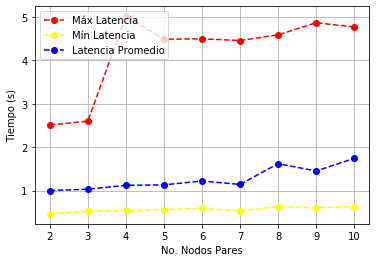
\includegraphics[scale=0.35]{Graphics/AnalisisLatenciaPares10TPSBS10.png}
\end{minipage}
}
\subfigure[Tama\~no de bloque igual 50.]{
\begin{minipage}[t]{0.30\linewidth}
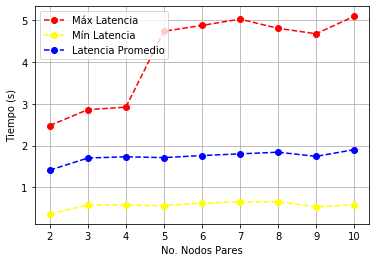
\includegraphics[scale=0.35]{Graphics/AnalisisLatenciaPares10TPSBS50.png}
\end{minipage}
}
\subfigure[Tama\~no de bloque igual 100.]{
\begin{minipage}[t]{0.30\linewidth}
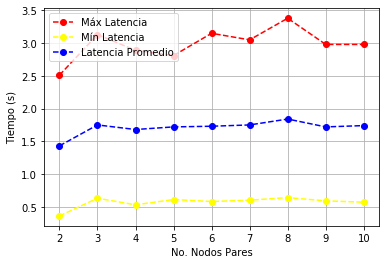
\includegraphics[scale=0.35]{Graphics/AnalisisLatenciaPares10TPSBS100.png}
\end{minipage}
}
\caption{Latencia en distintas configuraciones de nodos pares en una red con un solo nodo ordenador para escenarios de 10 TPS.}
\end{figure}

De acuerdo a la latencia m\'inima, para los tres casos mantienen un comportamiento similar, marcado por una leve tendencia al crecimiento con el aumento del n\'umero de nodos pares en la red. En el caso de la red configurada con un tama\~no de bloque igual a 10, los valores de latencia promedio son m\'as pr\'oximos a los valores de latencia m\'inima con respecto a las dem\'as configuraciones. Esto sucede porque al llegar las transacciones al servicio de ordenaci\'on, como el tama\~no del bloque es menor que el resto, y a su vez tiene una capacidad no superior al n\'umero de transacciones suministradas por los clientes, el tiempo de espera, en promedio, de las transacciones v\'alidas para cerrar el bloque es menor. Esta afirmaci\'on contrasta con la latencia m\'axima que, a menor tama\~no de bloques, mayores valores alcanza producto a que ocurre un proceso de llenado m\'as r\'apido originando una validaci\'on m\'as frecuente en los nodos pares, que a su vez participan en el proceso de simulaci\'on de las transacciones elevando la probabilidad de saturaci\'on en su proceso de ejecuci\'on.\\

En la figura \ref{ComparacionLatencia10TPS} se percibe que para un tama\~no de bloque igual a 10, el valor de latencia promedio es m\'inimo para todos las configuraciones de nodos pares. Luego, el tama\~no de bloque 10 es un par\'ametro que optimiza la latencia promedio en la red, en comparaci\'on a los dem\'as, por tanto, es un posible candidato a \'optimo.\\

\begin{figure}[h]
\centering
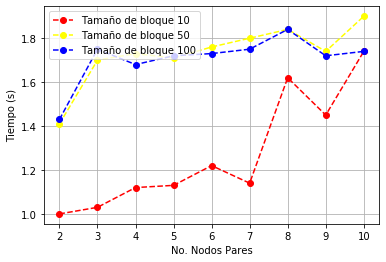
\includegraphics[scale=0.5]{Graphics/ComparacionLatencia10TPS.png}
\caption{Latencia promedio en redes con distinto tama\~no de bloque para escenarios de 10 TPS.}
\label{ComparacionLatencia10TPS}
\end{figure}


\subsection{An\'alisis de rendimiento}

\begin{figure}[h]
\subfigure[Tama\~no de bloque igual 10.]{
\begin{minipage}[t]{0.30\linewidth}
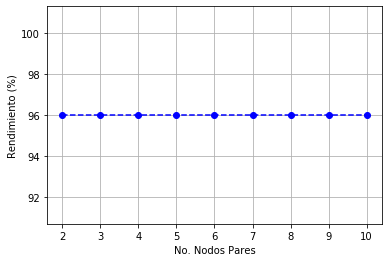
\includegraphics[scale=0.35]{Graphics/RendimientoPares10TPSBS10.png}
\end{minipage}
}
\subfigure[Tama\~no de bloque igual 50.]{
\begin{minipage}[t]{0.30\linewidth}
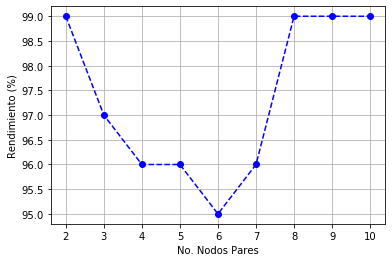
\includegraphics[scale=0.35]{Graphics/RendimientoPares10TPSBS50.png}
\end{minipage}
}
\subfigure[Tama\~no de bloque igual 100.]{
\begin{minipage}[t]{0.30\linewidth}
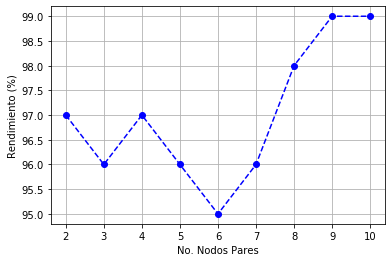
\includegraphics[scale=0.35]{Graphics/RendimientoPares10TPSBS100.png}
\end{minipage}
}
\caption{Rendimiento en distintas configuraciones de nodos pares en una red con un solo nodo ordenador para escenarios de 10 TPS.}
\end{figure}


Para los tama\~no de bloque planteados, los valores de rendimiento de la red oscilan entre el 95$\%$ y 99$\%$. La red configurada con tama\~no de bloque 10 mantiene un rendimiento constante de 96$\%$ para las configuraciones de nodos pares estudiadas.\\

 En el caso de la red con bloques de tama\~no 50 se alcanza un mejor rendimiento en la mayor\'ia de las configuraciones de nodos pares, como se puede ver en la figura \ref{RendimientoPares10TPS}.\\

\begin{figure}[h]
\centering
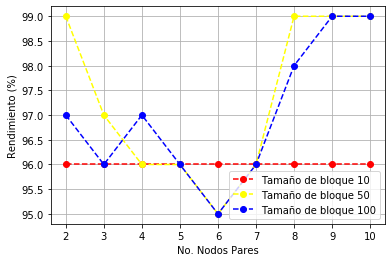
\includegraphics[scale=0.5]{Graphics/RendimientoPares10TPS.png}
\caption{Rendimiento de redes con distinto tama\~no de bloque para escenarios de 10 TPS.}
\label{RendimientoPares10TPS}
\end{figure}

\newpage

Para determinar una configuraci\'on \'optima, en relaci\'on a los valores de par\'ametros estudiados, se tuvo en cuenta el rendimiento en la red y la latencia promedio. Para establecer una comparaci\'on se llevaron las m\'etricas a una escala global, normalizando sus valores. Estos valores son estimaciones promedio para configuraciones con una cantidad de nodos pares entre dos y diez por organizaci\'on, donde el tama\~no en los bloques representa el factor a optimizar. En la figura \ref{Resultado10TPS} podemos ver que el mejor rendimiento se alcanza para canales con tama\~no de bloque igual a 50, pero a su vez la latencia promedio es mayor que la estimada para las configuraciones de canales de tama\~no 10. Por tanto, los valores 10 y 50 representan \'optimos locales, que en dependencia del escenario de uso, minimizan la latencia promedio y maximizan el rendimiento de la red respectivamente.\\

\begin{figure}[h]
\centering
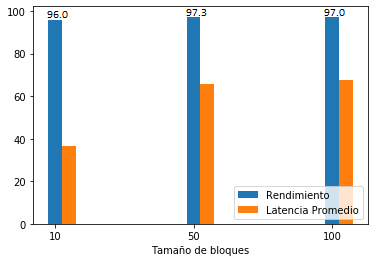
\includegraphics[scale=0.7]{Graphics/Resultado10TPS.png}
\caption{Evaluaci\'on de resultados para escenarios de 10 TPS.}
\label{Resultado10TPS}
\end{figure}

\newpage

\section{Escenario de alto volumen de transacciones}

En las tablas \ref{tab:100TPS-10BS}, \ref{tab:100TPS-50BS} y \ref{tab:100TPS-100BS} se registran los datos obtenidos para el escenario de 100 TPS.\\

\subsection{An\'alisis de latencia}

Las siguientes gr\'aficas muestran el comportamiento de la latencia promedio en la red configurada con cada tama\~no de bloque estudiado.\\

\begin{figure}[htbp]
\subfigure[Tama\~no de bloque igual 10.]{
\begin{minipage}[t]{0.30\linewidth}
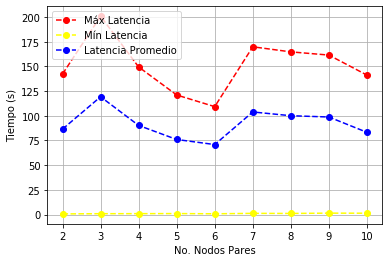
\includegraphics[scale=0.35]{Graphics/AnalisisLatenciaPares100TPSBS10.png}
\end{minipage}
}
\subfigure[Tama\~no de bloque igual 50.]{
\begin{minipage}[t]{0.30\linewidth}
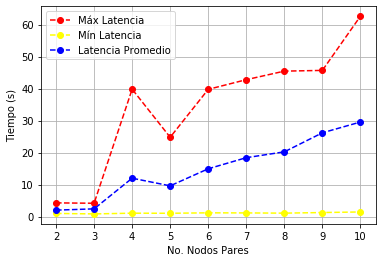
\includegraphics[scale=0.35]{Graphics/AnalisisLatenciaPares100TPSBS50.png}
\end{minipage}
}
\subfigure[Tama\~no de bloque igual 100.]{
\begin{minipage}[t]{0.30\linewidth}
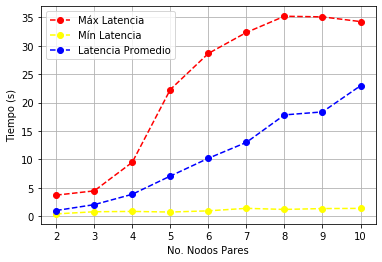
\includegraphics[scale=0.35]{Graphics/AnalisisLatenciaPares100TPSBS100.png}
\end{minipage}
}
\caption{Latencia en distintas configuraciones de nodos pares en una red con un solo nodo ordenador para escenarios de 100 TPS.}
\end{figure}


En la primera gr\'afica podemos observar que los valores de latencia promedio oscilan entre los 70 y 120 segundos aproximadamente. Estos valores son, en extremo, elevados en comparaci\'on con las restantes configuraciones. Para el caso de los bloques de tama\~no 100 el mayor valor alcanzado de latencia promedio, no supera los 25 segundos, quedando todos sus valores por debajo de los alcanzados por la configuraci\'on de bloques de tama\~no 10. Lo mismo sucede en las redes con bloques de tama\~no 50 que no superan los 30 segundos.\\

Para determinar el tama\~no de bloque que ofrece mejor desempe\~no en redes con un n\'umero de nodos pares que var\'ia de dos a diez por organizaci\'on,  con respecto a la latencia de las transacciones, se calcul\'o la media de las latencias promedios de las configuraciones de nodos pares, por tama\~nos de bloques, y nos quedamos con la configuraci\'on de bloque que corresponda a la menor de ellas.\\

Los bloques de tama\~no 10, 50 y 100 promedian una latencia media para las configuraciones de nodos pares de 92.1, 15.0 y 10.7 segundos respectivamente. Por tanto, las redes configuradas con bloques de tama\~no 100 son \'optimas respecto al conjunto estudiado, propiciando la menor latencia promedio. Para establecer una comparativa visual nos podemos remitir a la figura \ref{ComparacionLatencia100TPS}.\\

\begin{figure}[h]
\centering
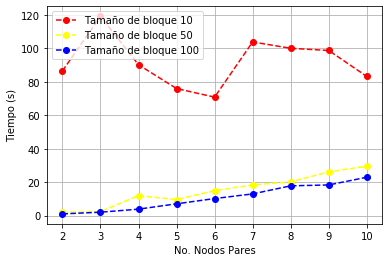
\includegraphics[scale=0.5]{Graphics/ComparacionLatencia100TPS.png}
\caption{Latencia promedio en redes con distinto tama\~no de bloque para escenarios de 100 TPS.}
\label{ComparacionLatencia100TPS}
\end{figure}

\subsection{An\'alisis de rendimiento}

\begin{figure}[h]
\subfigure[Tama\~no de bloque igual 10.]{
\begin{minipage}[t]{0.30\linewidth}
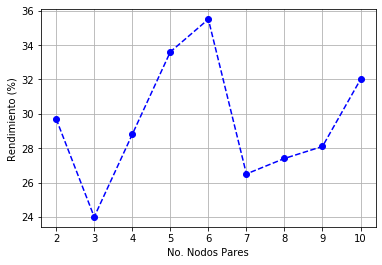
\includegraphics[scale=0.35]{Graphics/RendimientoPares100TPSBS10.png}
\end{minipage}
}
\subfigure[Tama\~no de bloque igual 50.]{
\begin{minipage}[t]{0.30\linewidth}
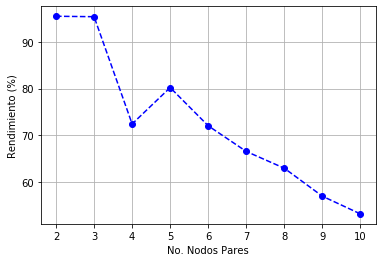
\includegraphics[scale=0.35]{Graphics/RendimientoPares100TPSBS50.png}
\end{minipage}
}
\subfigure[Tama\~no de bloque igual 100.]{
\begin{minipage}[t]{0.30\linewidth}
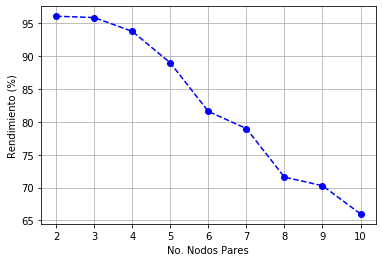
\includegraphics[scale=0.35]{Graphics/RendimientoPares100TPSBS100.png}
\end{minipage}
}
\caption{Rendimiento en distintas configuraciones de nodos pares en una red con un solo nodo ordenador para escenarios de 100 TPS.}
\end{figure}

De acuerdo a la gr\'afica que representa el rendimiento para las redes con bloques de tama\~no 10, se destaca el bajo rendimiento que logran en escenarios de altos vol\'umenes de transacciones. Entre las causas fundamentales que lo ocasionan est\'a el r\'apido llenado de los bloques por el servicio de ordenaci\'on, que luego son enviados, con mayor frecuencia, a los nodos pares para el proceso de validaci\'on y a su vez se conjuga con el alto volumen de transacciones que deben simular en cada intervalo de tiempo. Los bloques de tama\~no 50 y 100 manifiestan un mejor rendimiento debido a que compensan la frecuencia de validaci\'on por los nodos pares, con un aumento del tiempo de conformaci\'on de bloques.\\

Si ilustramos las curvas de rendimiento en una sola gr\'afica, como en la figura \ref{RendimientoPares100TPS}, apreciamos que las redes con bloques de tama\~no 100 superan para todas las configuraciones de nodos pares, a las redes con bloques de tama\~no inferior. Se aprecia adem\'as, que para escenarios de altos vol\'umenes de transacciones por segundo, el aumento del n\'umero de nodos pares en las organizaciones reducen el rendimiento de forma considerable.

\begin{figure}[h]
\centering
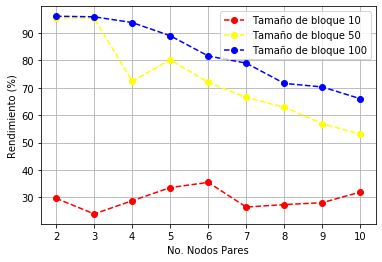
\includegraphics[scale=0.5]{Graphics/RendimientoPares100TPS.png}
\caption{Rendimiento de redes con distinto tama\~no de bloque para escenarios de 100 TPS.}
\label{RendimientoPares100TPS}
\end{figure}

En este escenario, la configuraci\'on para bloques de tama\~no 100, propicia la menor latencia promedio en la red y el mejor desempe\~no en el rendimiento, del conjunto evaluado. En la figura \ref{Resultado100TPS} se puede ver el marcado contraste dado por la diferencia en el tama\~no de los bloques. Se tiene una diferencia m\'axima de latencia superior a los 80 segundos, igual comportamiento tenemos en el rendimiento, donde los bloque de tama\~no 10 ofrecen las m\'etricas m\'as desfavorables. A su vez, esta coincide con la configuraci\'on, por defecto, de la red para los canales de comunicaci\'on. Por tanto, confirma la necesidad de evaluar los par\'ametros del sistema antes de su puesta en producci\'on.\\

\begin{figure}[h]
\centering
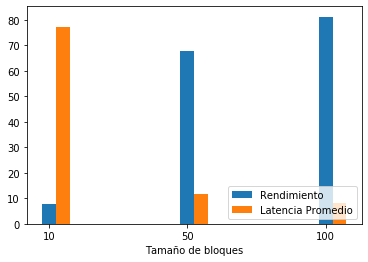
\includegraphics[scale=0.6]{Graphics/Resultado100TPS.png}
\caption{Evaluaci\'on de resultados para escenarios de 100 TPS.}
\label{Resultado100TPS}
\end{figure}

%\section*{An\'alisis de la influencia de los nodos pares y ordenadores en los escenarios estudiados}


\backmatter

\begin{conclusions}
    Conclusiones
\end{conclusions}

\begin{recomendations}
El estudio se realiz\'o sobre una muestra de par\'ametros de configuraci\'on, y se determin\'o con respecto a ellos, los que optimizan escenarios de 10 y 100 transacciones por segundo. Propongo extender la investigaci\'on para una muestra de tama\~no mayor, que permita realizar un an\'alisis en pruebas de hip\'otesis para tratar de obtener una generaliaci\'on en el comportamiento de la variaci\'on de los par\'ametros.\\

Determinar un tama\~no adecuado de los bloques en un canal de comunicaci\'on, resulta una tarea compleja producto a la influencia directa que tiene sobre varias de las componentes de fabric, como los nodos pares y los nodos ordenadores. Por lo que trabajar en una herramienta que itere de manera eficiente para converger hacia un posible candidato a tama\~no \'optimo ayudar\'ia en gran medida a encontrar los valores que mejoren el rendimiento en un escenario determinado.
\end{recomendations}

\printbibliography[heading=bibintoc]


\end{document}
